
% This LaTeX was auto-generated from an M-file by MATLAB.
% To make changes, update the M-file and republish this document.

\documentclass{article}
\usepackage{graphicx}
\usepackage{color}

\sloppy
\definecolor{lightgray}{gray}{0.5}
\setlength{\parindent}{10pt}
\usepackage[margin=1in]{geometry}

\begin{document}

\title{Dynamical Adaptation in ORNs}
\author{Srinivas Gorur-Shandilya}
\maketitle

    
    
\subsection*{Contents}

\begin{itemize}
\setlength{\itemsep}{-1ex}
   \item Do ORNs rapidly modulate gain?
   \item Sanity check: Linear synthetic data vs. linear gain analysis
   \item Synthetic Data: DA Model vs. Linear Gain Analysis
   \item Synthetic Data: DA Model with exp. gaussian inputs vs. Linear Gain Analysis
\end{itemize}


\subsection*{Do ORNs rapidly modulate gain?}

\begin{par}
Pseudo-white-noise analysis of ORN responses involves presenting binary flickering pulses of odor to the ORN and recording their response. If ORNs rapidly modulate gain on the timescale of response, then responses to pulses of odor in the sequence where the stimulus is locally low will be different from responses to pulses of odor in the sequence where the stimulus is locally high.
\end{par} \vspace{1em}
\begin{par}
The data looks like this. The following figure shows the valve state, the odor concentration, and the neuron response. The neuron is ab3A, and the odor presented is 1-octen-3-ol diluted to 3x $10^{-3}$ in Paraffin Oil. The correlation time in the valve position is 30ms.
\end{par} \vspace{1em}
\begin{par}
This data file is used for the following analysis:
\end{par} \vspace{1em}

        \color{lightgray} \begin{verbatim}final_2011_06_14_ab3A_1o3ol3X-3_20ml_30sec_30ms_rand.mat
\end{verbatim} \color{black}
    
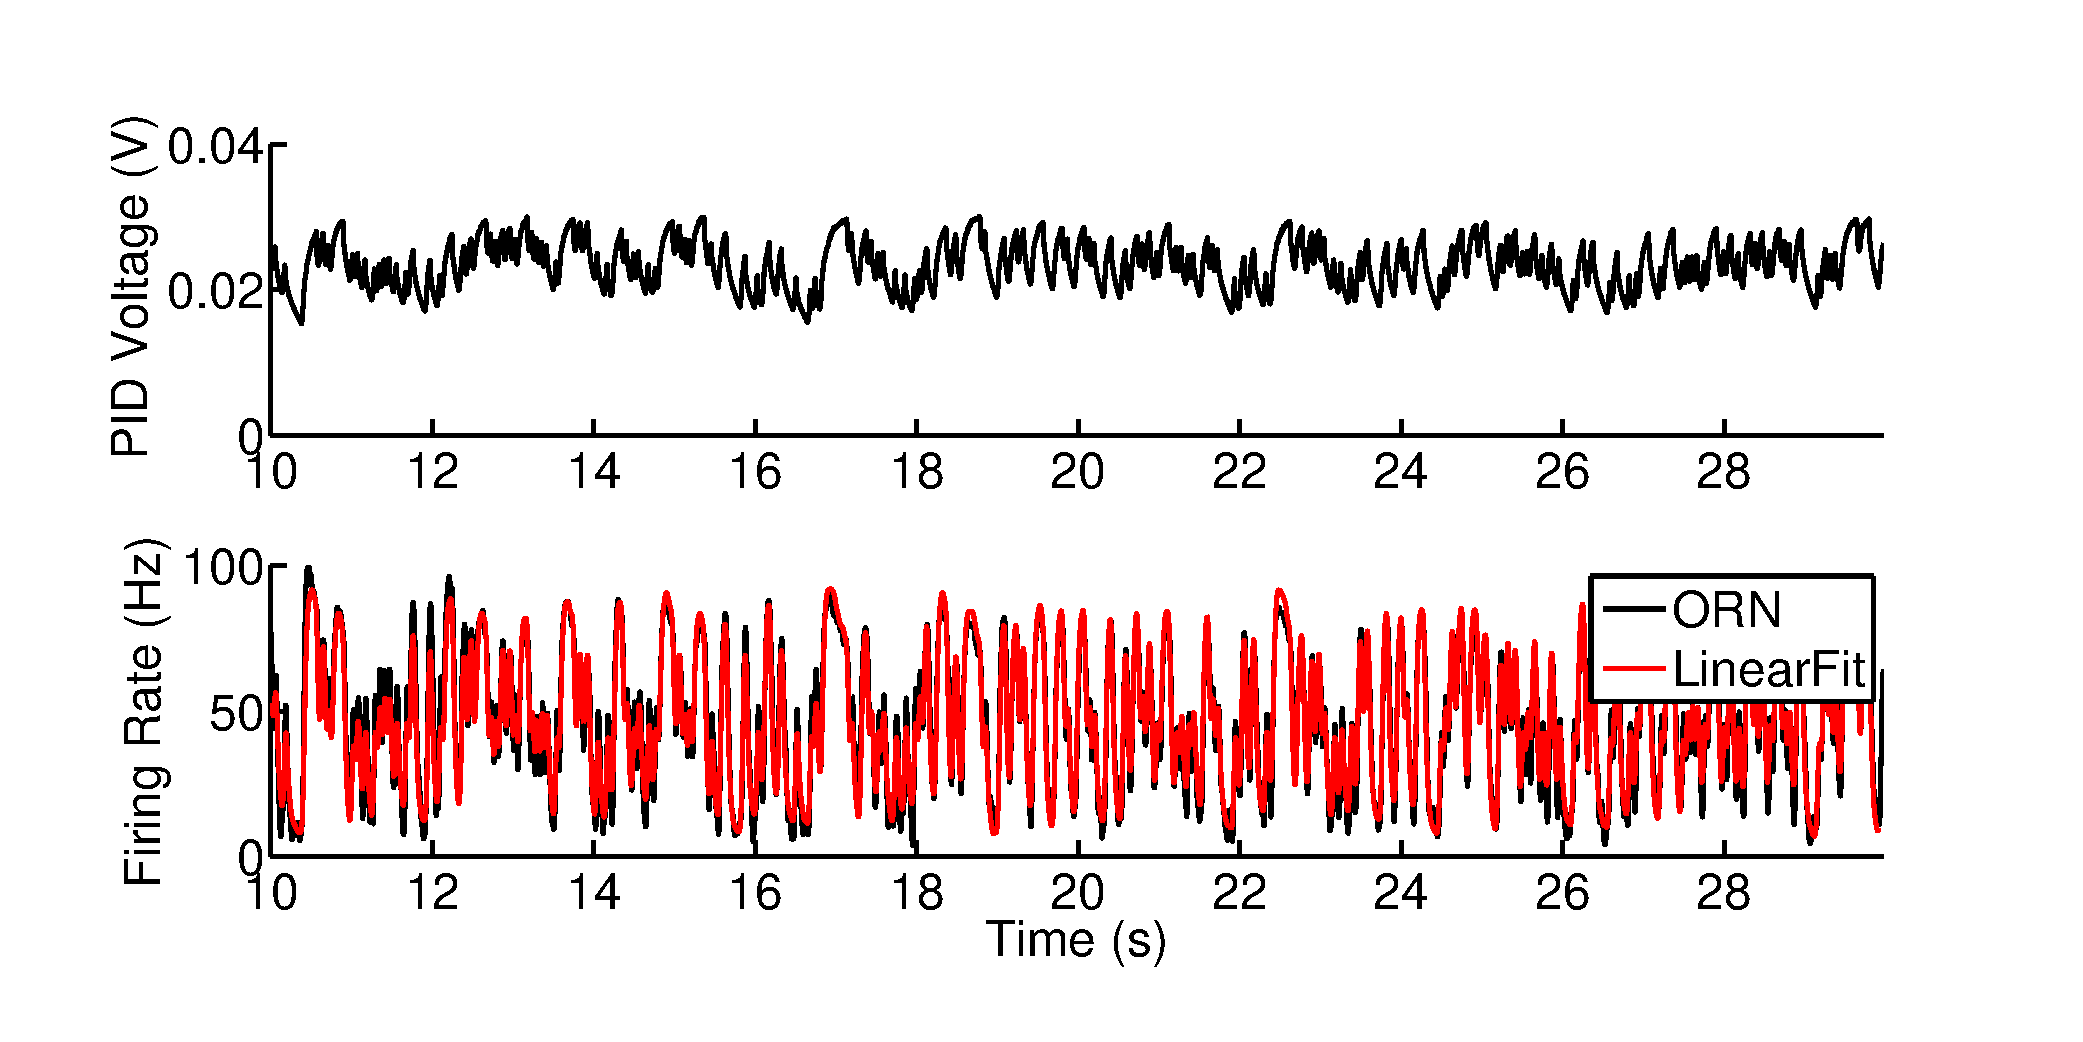
\includegraphics [width=\textwidth]{Understanding_Linear_Gain_Analysis_01.pdf}

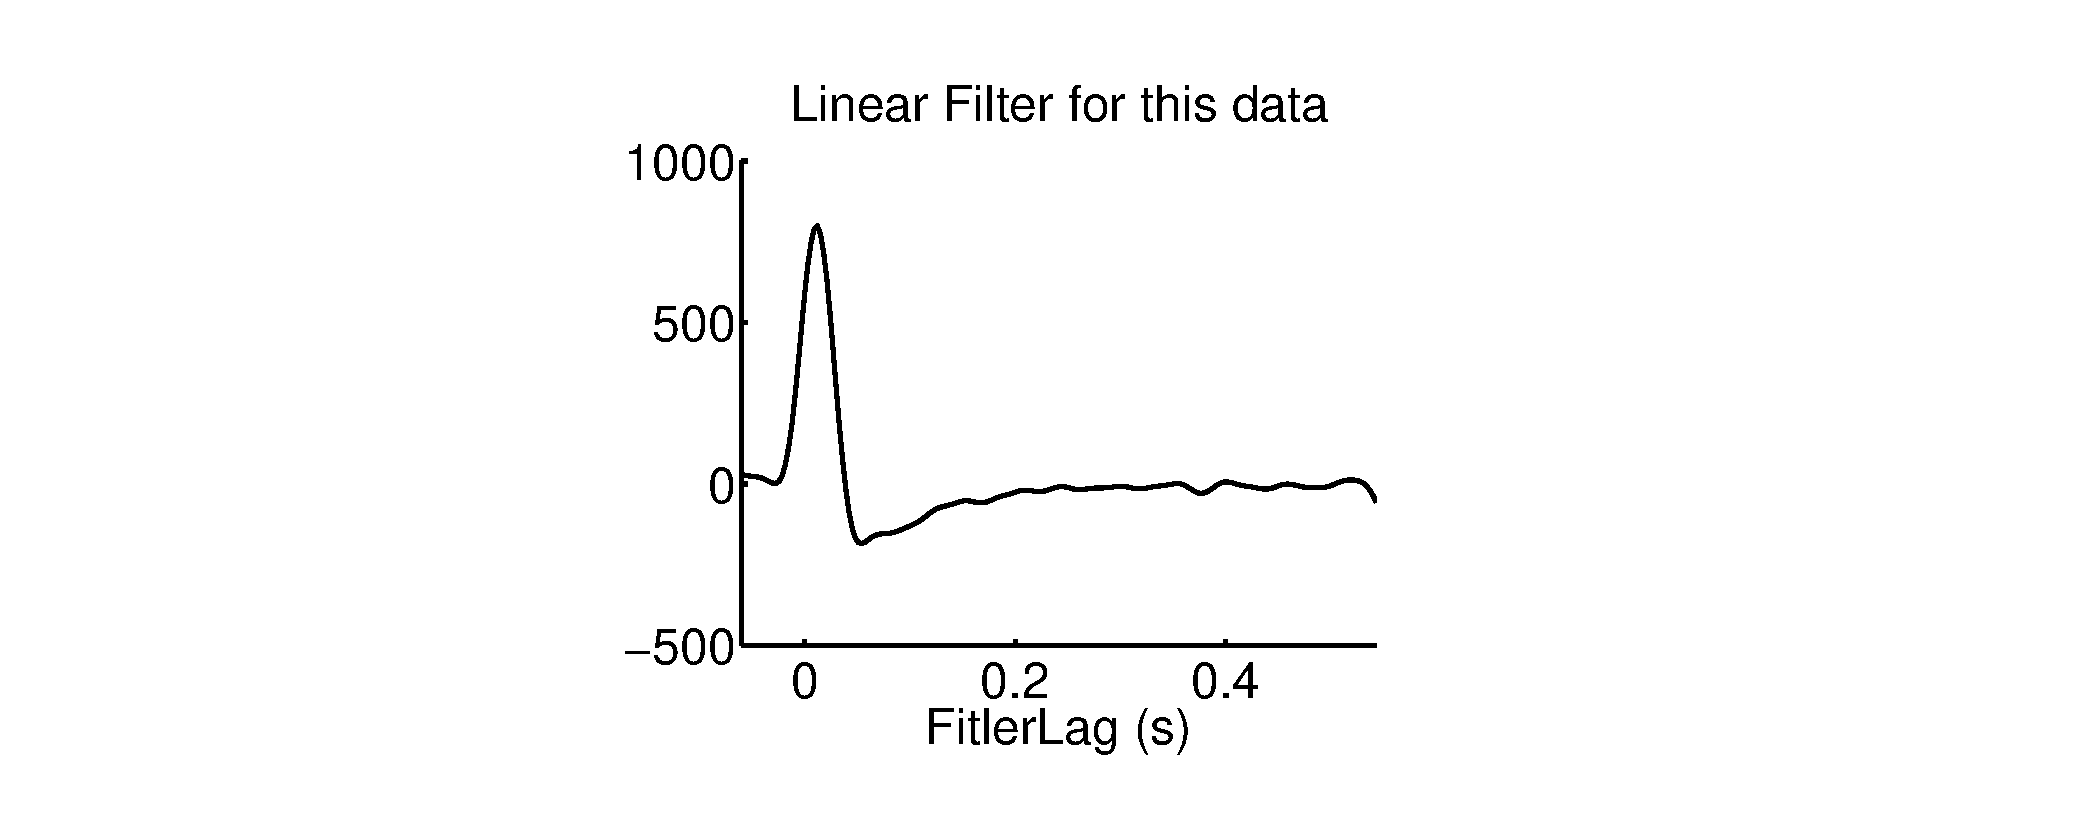
\includegraphics [width=\textwidth]{Understanding_Linear_Gain_Analysis_02.pdf}
\begin{par}
The distributions of the input to neuron and the neuron responses are shown below on the left. The autocorrelaiton functions of the input and output are shown on the right. If the ORN modulates its gain on a rapid time-scale, it must do so in this case on a time-scale smaller than the autocorrelation time of the stimulus.
\end{par} \vspace{1em}

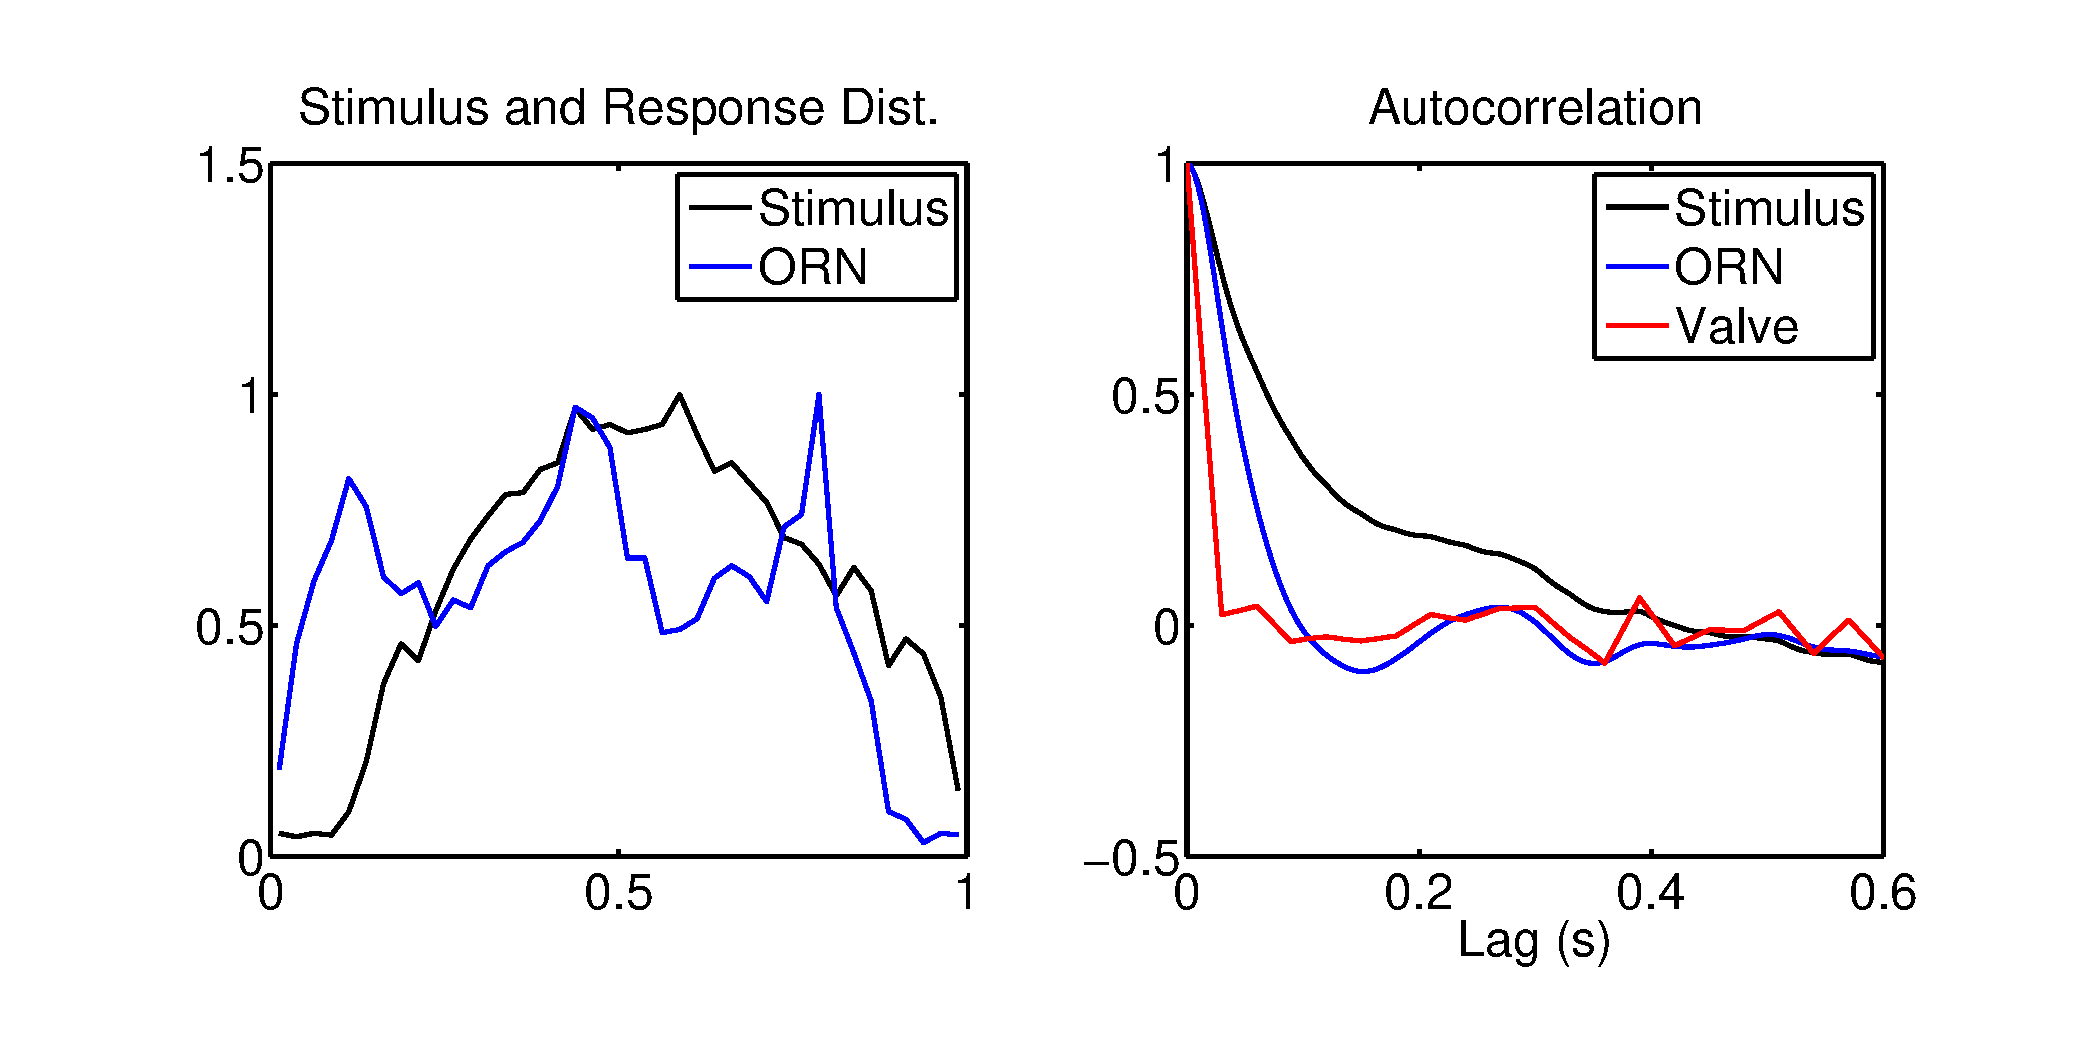
\includegraphics [width=\textwidth]{Understanding_Linear_Gain_Analysis_03.pdf}
\begin{par}
Does the ORN selectively amplify responses to relatively small stimuli and suppress responses to relatively high stimuli?
\end{par} \vspace{1em}

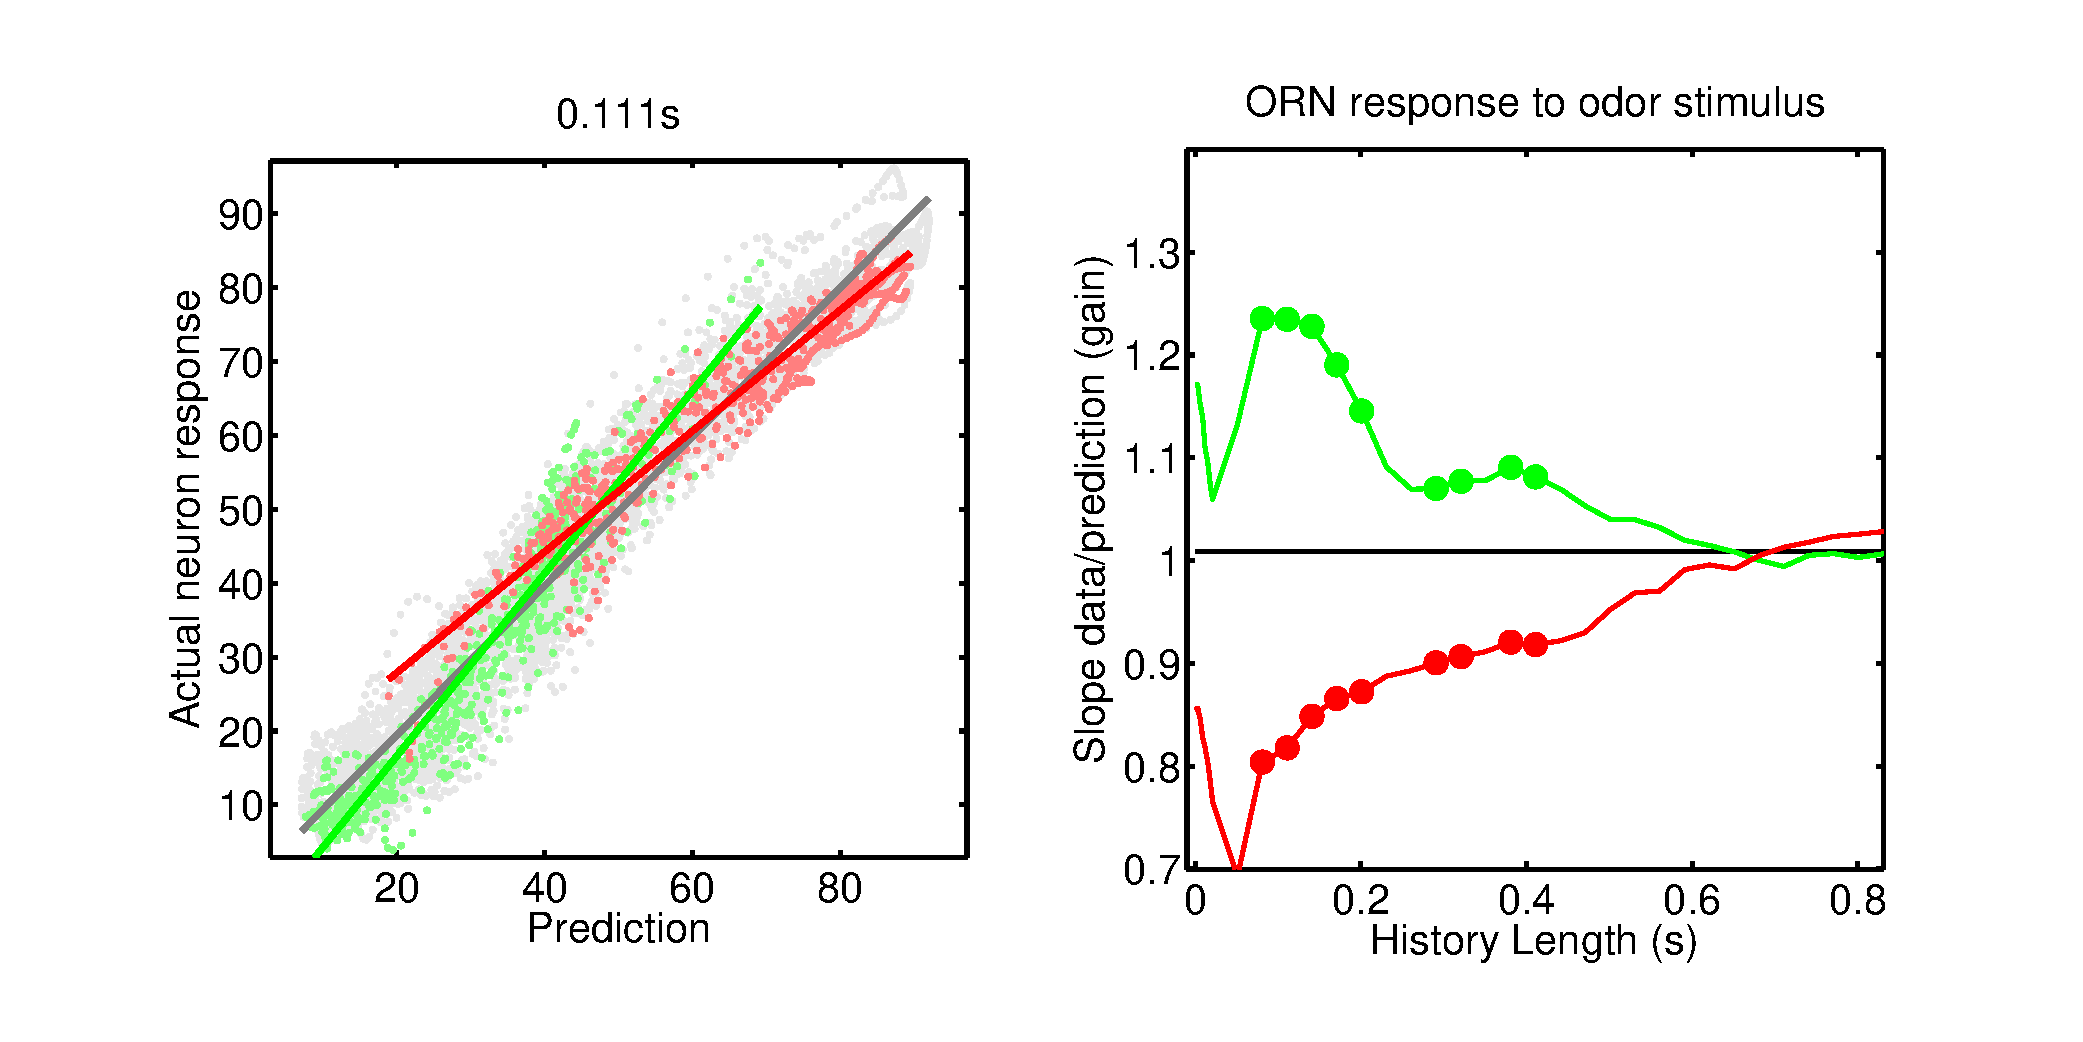
\includegraphics [width=\textwidth]{Understanding_Linear_Gain_Analysis_04.pdf}
\begin{par}
The gain as a function of history length is pretty weird. Why does it not go to 1 when history length is 0? Why is there a mysterious downward deflection close to 0?
\end{par} \vspace{1em}


\subsection*{Sanity check: Linear synthetic data vs. linear gain analysis}

\begin{par}
To figure this out, let's first repeat the gain analysis, but instead of using the ORN response, we use the linear prediction itself.
\end{par} \vspace{1em}

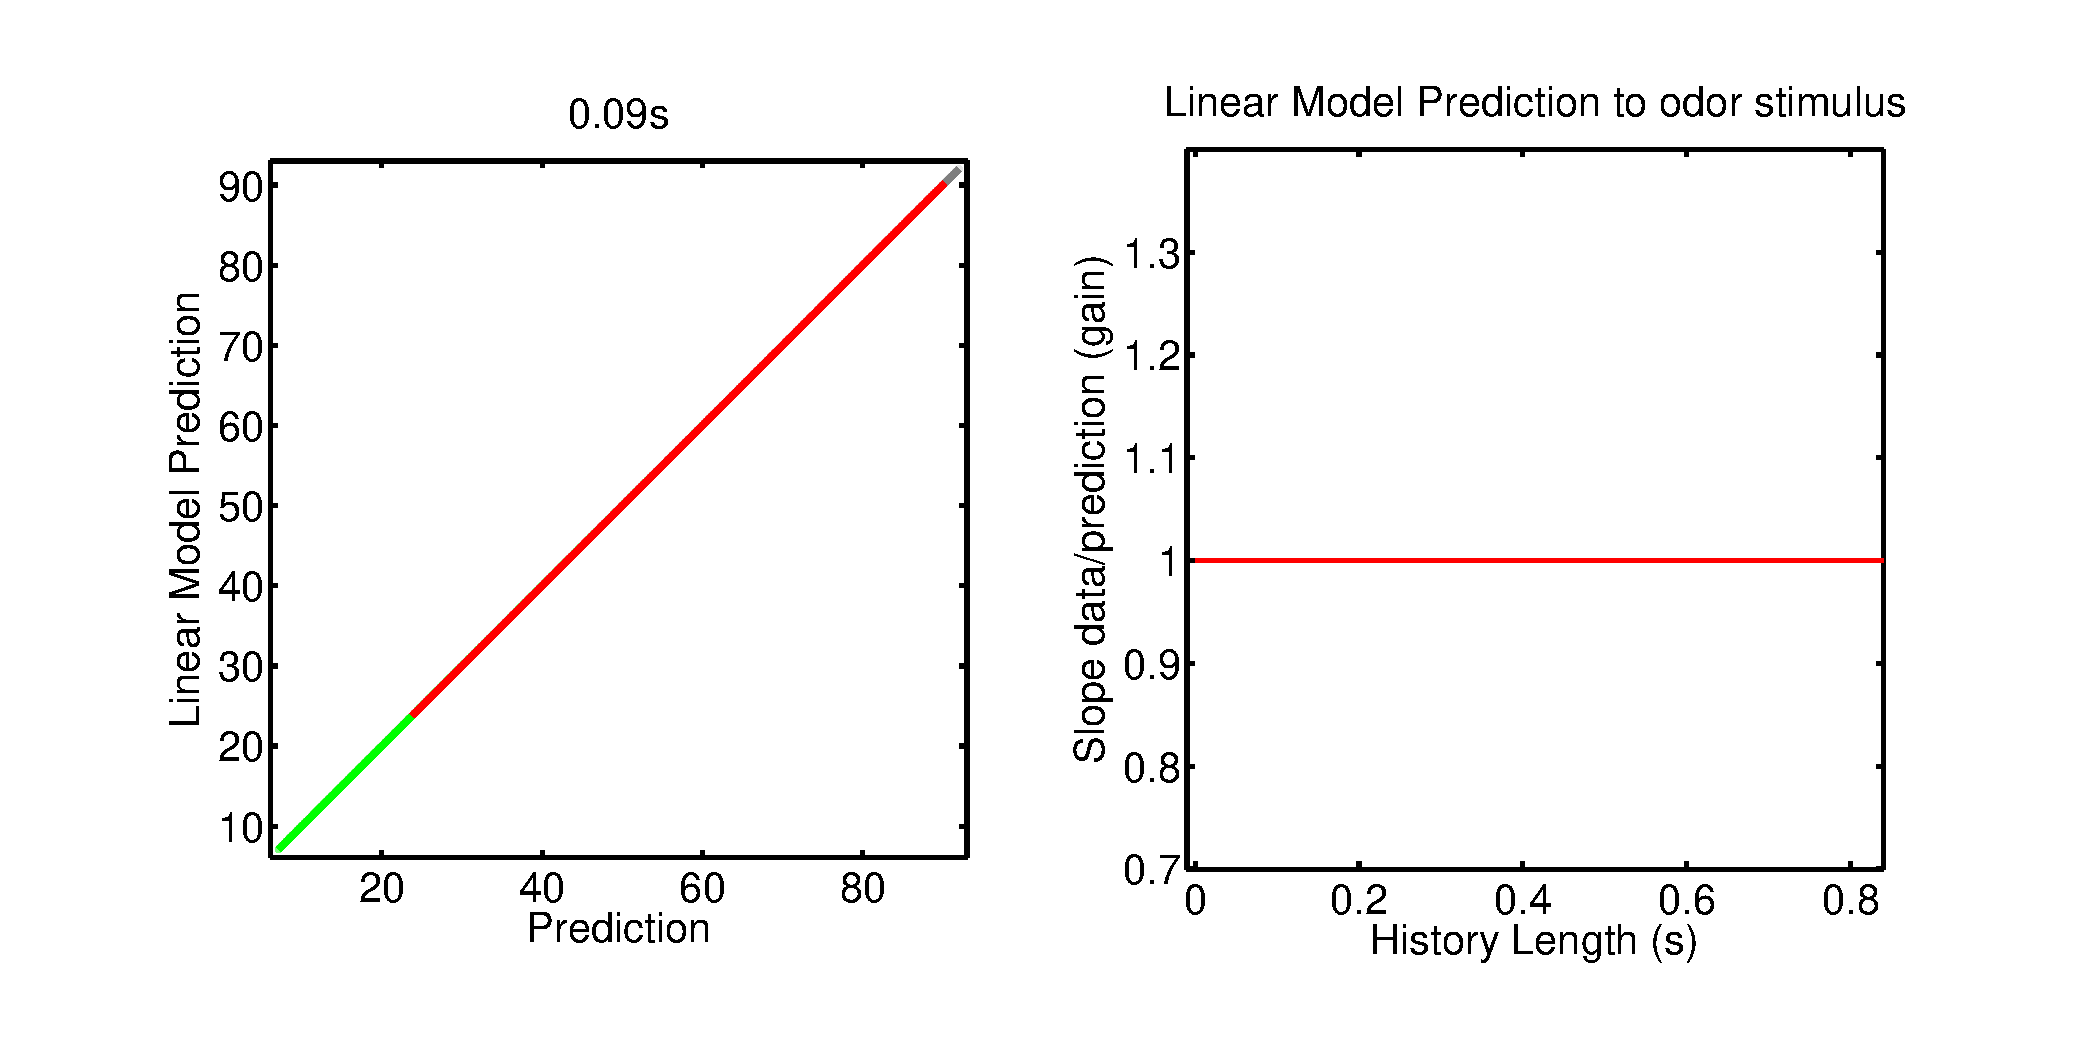
\includegraphics [width=\textwidth]{Understanding_Linear_Gain_Analysis_05.pdf}


\subsection*{Synthetic Data: DA Model vs. Linear Gain Analysis}

\begin{par}
Do we still see the weird behaviour of the slope plots with synthetic data? Here we generate the synthetic neuron data by using a DA model to simulate neuron output, with parameters roughly chosen to somewhat match actual ORN statistics.
\end{par} \vspace{1em}

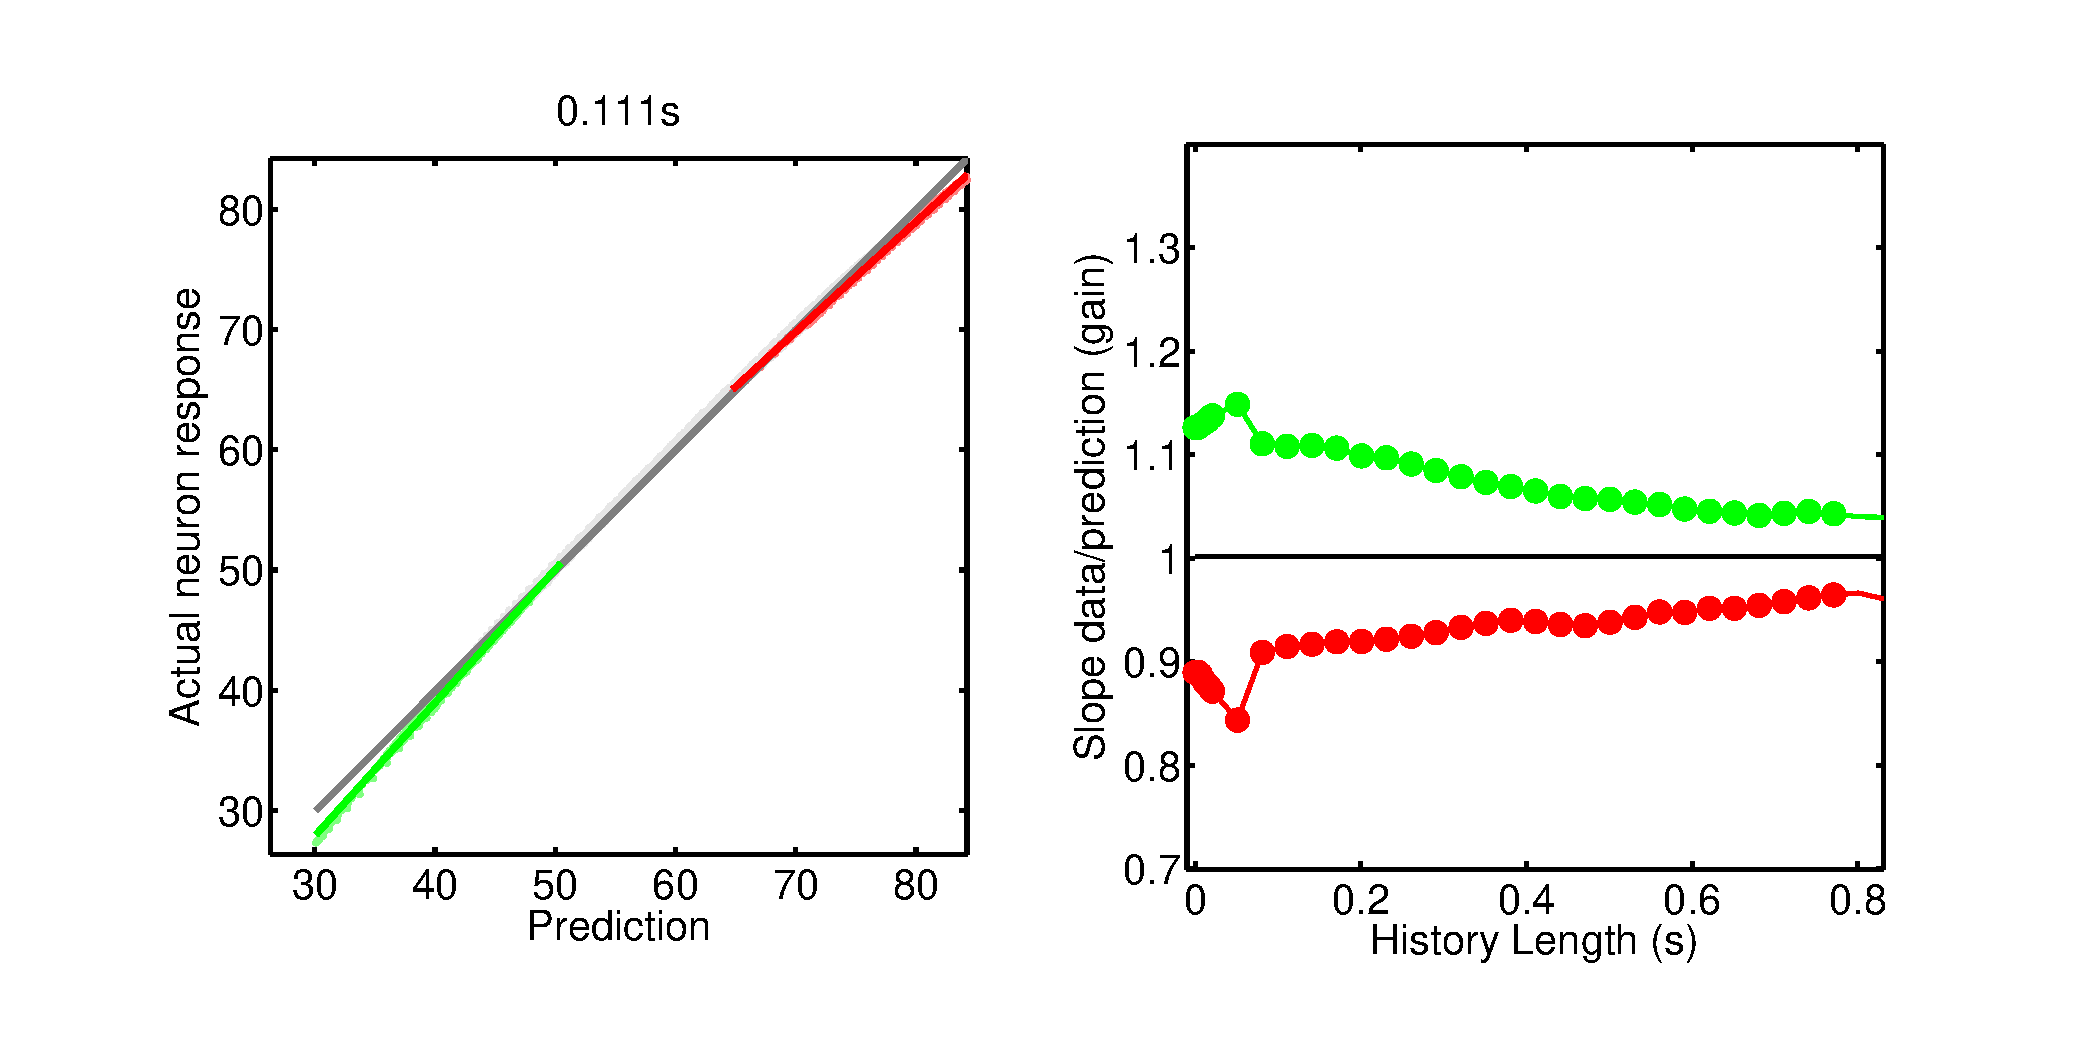
\includegraphics [width=\textwidth]{Understanding_Linear_Gain_Analysis_06.pdf}


\subsection*{Synthetic Data: DA Model with exp. gaussian inputs vs. Linear Gain Analysis}

\begin{par}
So we still see this weird thing. Maybe it's because of something in the stimulus? Now we use the same model but now feed it with exponentiated Gaussian inputs.
\end{par} \vspace{1em}

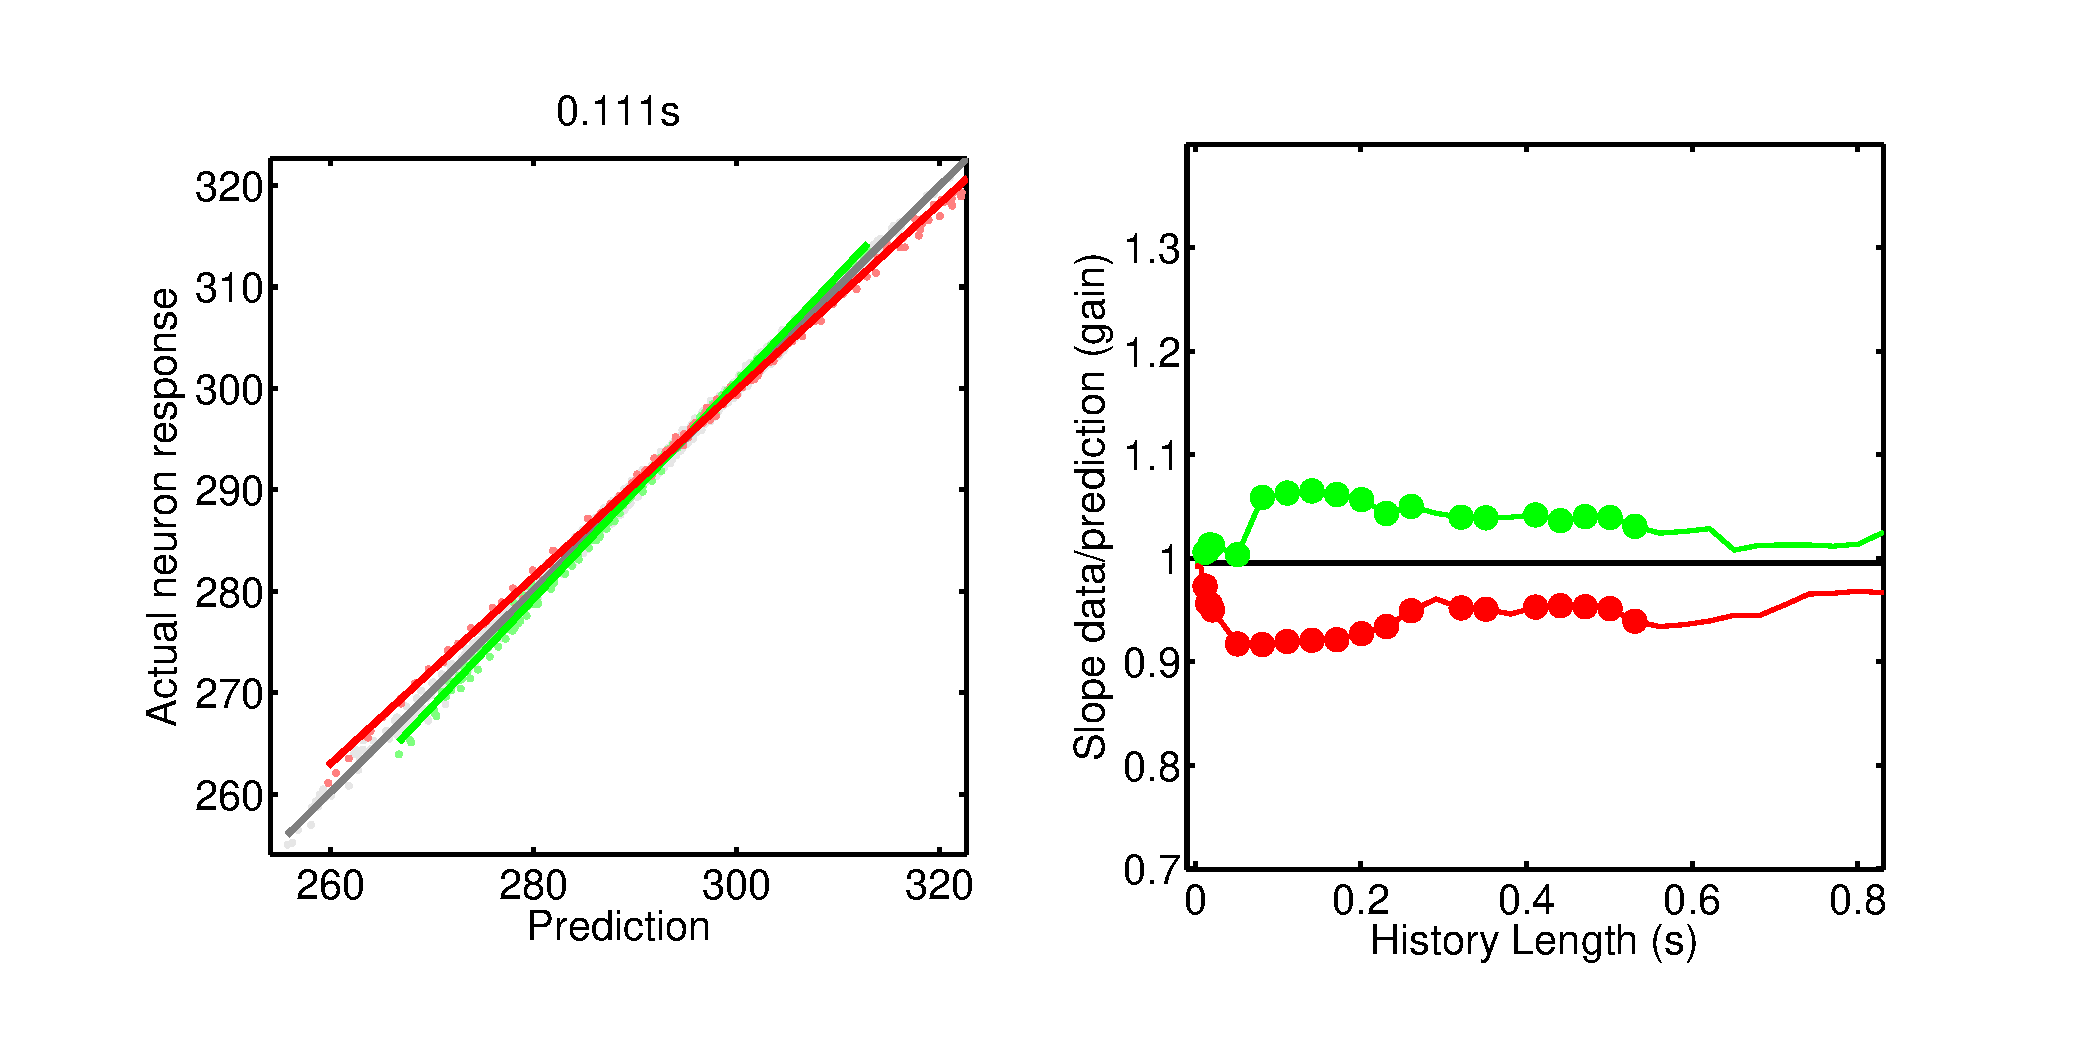
\includegraphics [width=\textwidth]{Understanding_Linear_Gain_Analysis_07.pdf}
\begin{par}
OK, now the slopes go to unity as the history length goes to 0. What about the stimulus causes the slopes not to go to 1? Perhaps filtering the stimulus makes this effect come back.
\end{par} \vspace{1em}

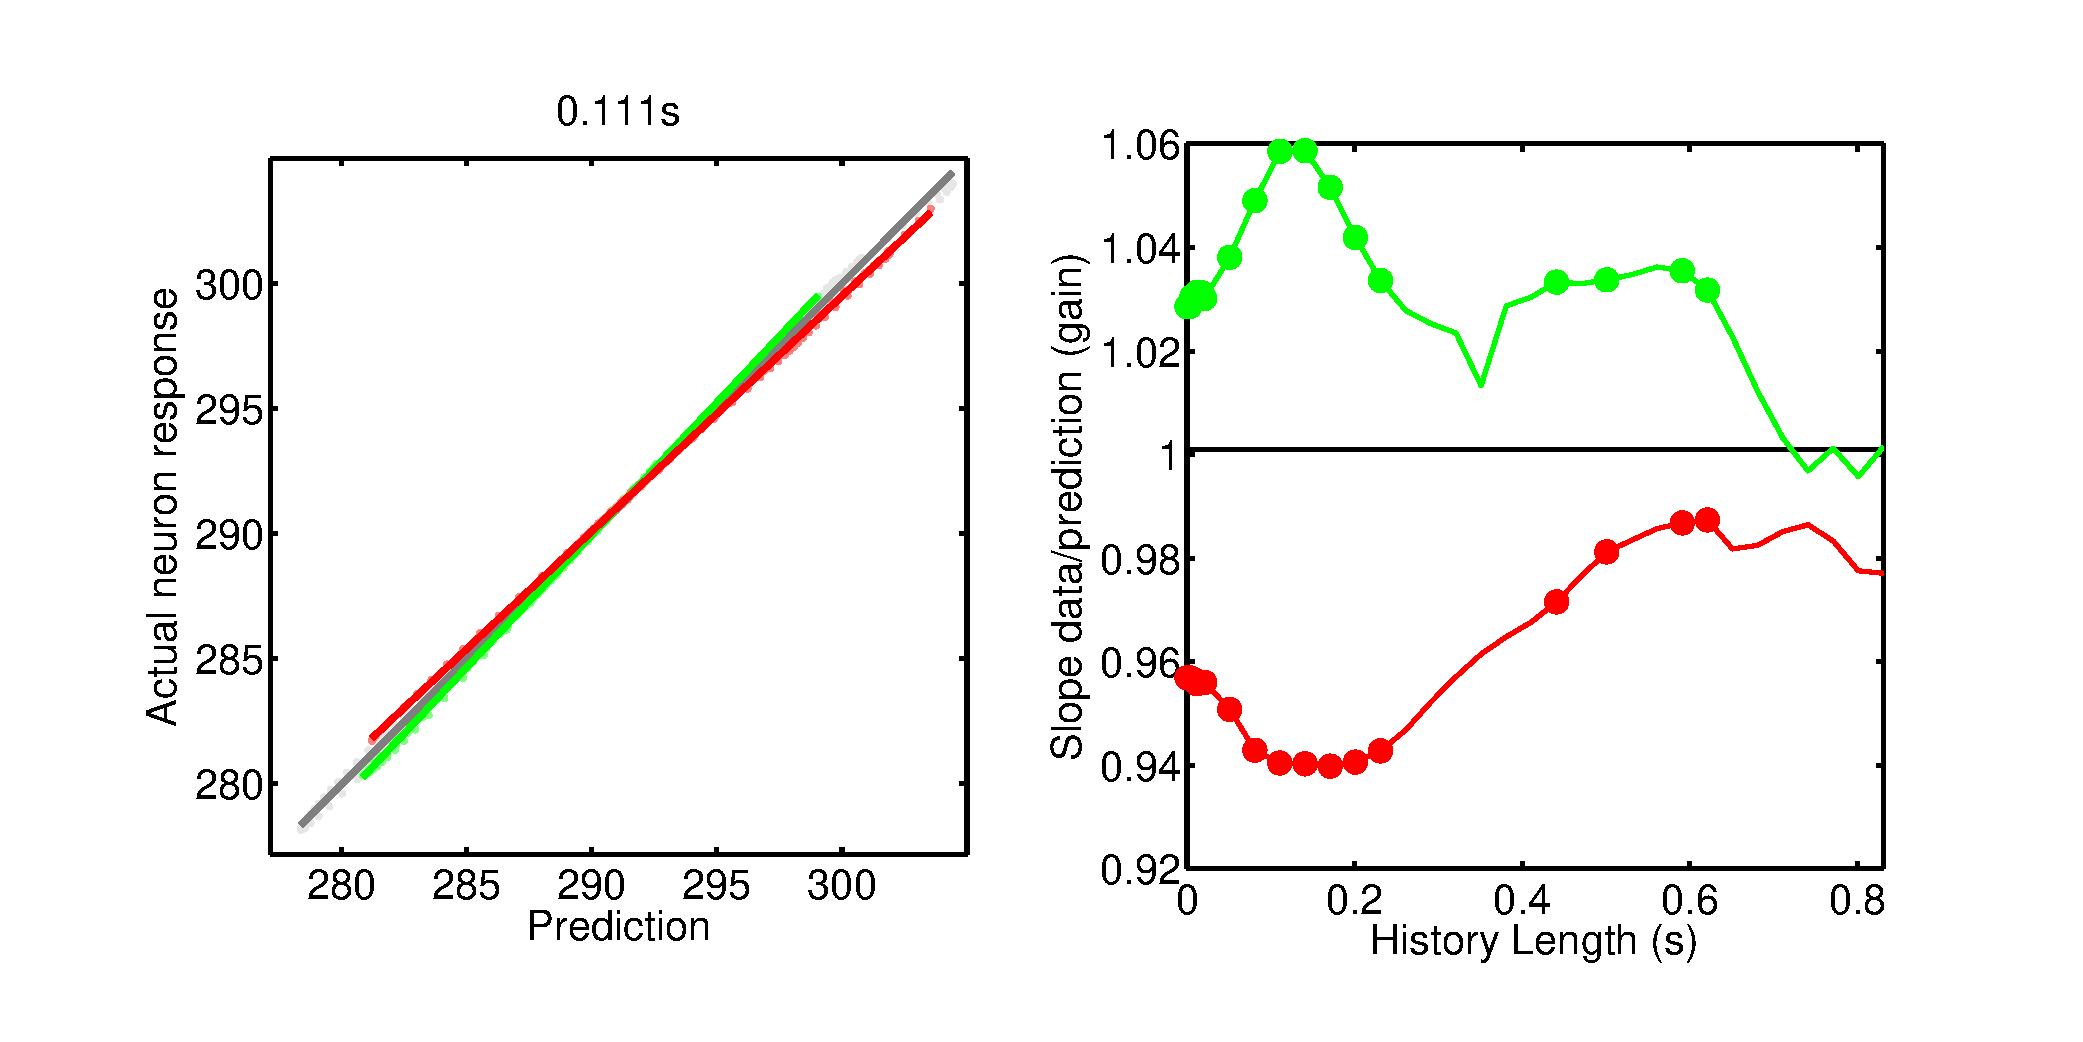
\includegraphics [width=\textwidth]{Understanding_Linear_Gain_Analysis_08.pdf}
\begin{par}
Why does this happen? Why do the gain slopes not go to zero when the history length is zero? This makes sense when we consider what the history length actually is. For varying history lengths, we choose varying smoothing windows and smooth the stimulus with this. However, when the history length is 0 in this case, this doesn't mean the stimulus is not being smoothed! Technically, it is being smoothed, already, as the stimulus itself has correlations.
\end{par} \vspace{1em}



\end{document}
    
